\documentclass[dvipsnames]{article}
\usepackage{pgfplots}
\usetikzlibrary{decorations.markings}
\pgfplotsset{compat=newest}

% \def\Point{36.9}

\begin{document}

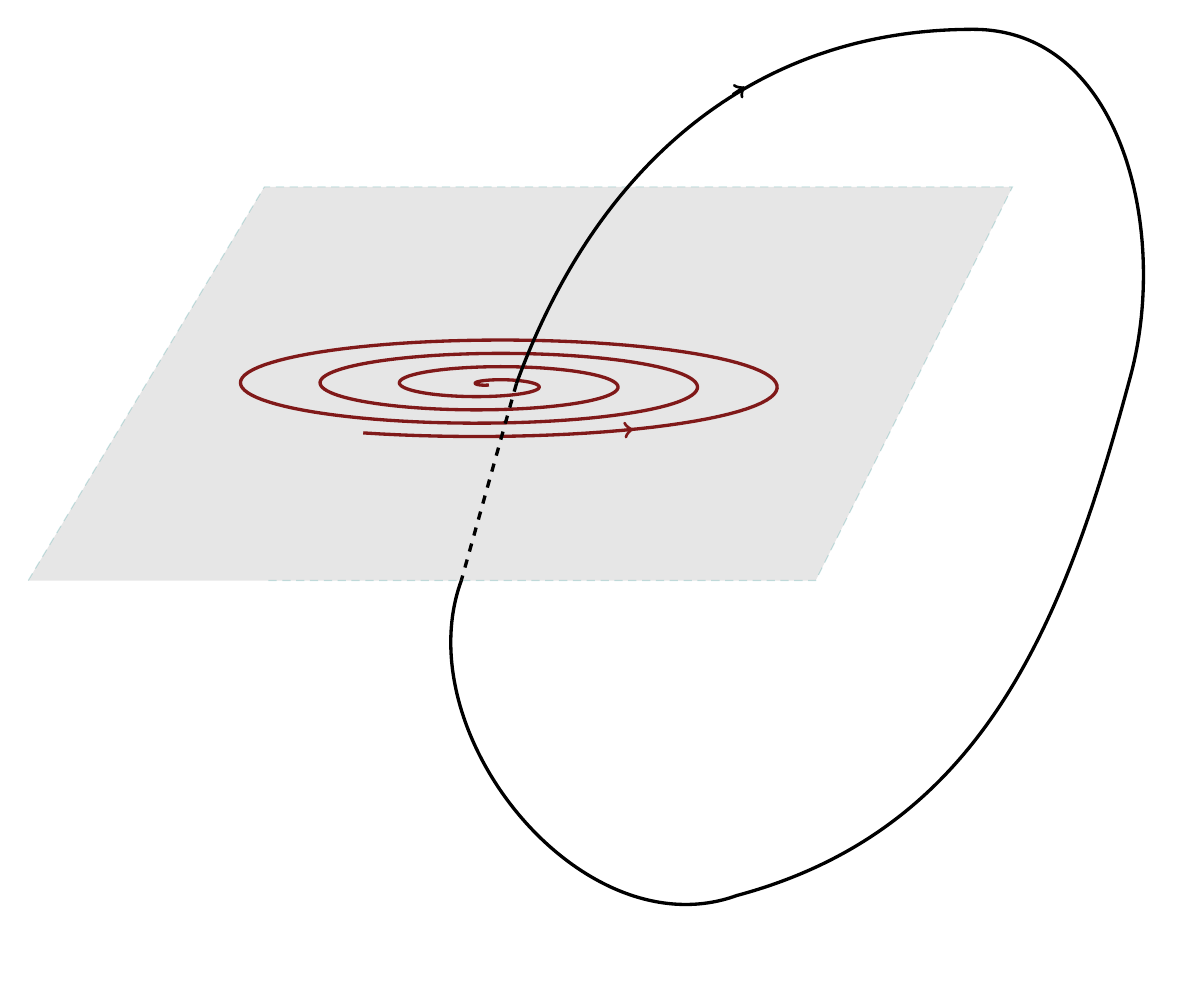
\begin{tikzpicture}
%левая
  \begin{axis}[
    view={-50}{-10}, %угол обзора
    axis lines=none,
    zmax=60,
    height=10cm,
    xtick=\empty,
    ytick=\empty,
    ztick=\empty
    ]
    
    %спираль
    \addplot3+[,ytick=\empty,yticklabel=\empty,
    mark=none,
    very thick,
    color={rgb,255:red,128; green,0; blue,0},
    domain=0:10*pi,
    postaction={decorate,
                decoration={markings,mark=at position 0.9 with {\arrow{<}}}
               },
    samples=400,
    samples y=0,
    ]
    (-{x*sin(0.25*pi*deg(x))},{x*cos(0.25*pi*deg(x)},{0});
    ]
  \end{axis}
  %плоскость
  \draw[teal,densely dashed][fill = gray, opacity=0.2]  (-1,-1) -- (2,4) -- (11.5,4) -- (9,-1) -- (2,-1);
  %цикл
  \draw[very thick, dashed]  (5.2,1.5) --(4.5,-1);
  \draw [very thick] (5.2,1.5) to [out=70,in=-180] (11,6) to [out=0,in=75] (13,1.6) to [out=-105,in=15] (8,-5) to [out=-160,in=-110] (4.5,-1);
  \draw[very thick] [->] (7.95,5.17) --(8.1,5.27);
\end{tikzpicture}
\end{document}